\documentclass{beamer}
\usetheme{Warsaw}

%% Lots of packages !
\usepackage{etex}

%% Francisation
\usepackage[francais]{babel}
\usepackage[T1]{fontenc}
\usepackage[utf8]{inputenc}
%\usepackage{textcomp}

%% Réglages généraux
\usepackage{setspace}
\usepackage{lscape}
%\usepackage{multicol}
\usepackage{makeidx}
%\usepackage[clearempty]{titlesec}
%\usepackage{cite}

%% Packages pour le texte
\usepackage{pifont}
\usepackage{eurosym}
\usepackage{soul}
\usepackage[normalem]{ulem}
\usepackage{fancybox}
\usepackage{boxedminipage}
\usepackage{enumerate}
\usepackage{verbatim}
\usepackage{moreverb}
\usepackage{listings}
%\usepackage[table]{xcolor}

%% Packages pour les tableaux
\usepackage{array}
\usepackage{multirow}
\usepackage{tabularx}
\usepackage{longtable}

%% Packages pour les dessins
\usepackage{graphicx}
\usepackage{wrapfig}
%\usepackage{picins}
\usepackage{picinpar}
\usepackage{epic}
\usepackage{eepic}
\usepackage{tikz}
\usepackage{afterpage}
\usepackage{rotating}
\usepackage{float}
\usepackage{caption}

%% Packages pour les maths
\usepackage{amsmath}
\usepackage{amssymb}
\usepackage{dsfont}
\usepackage{mathrsfs}
\usepackage{bussproofs}
%\usepackage[thmmarks,amsmath]{ntheorem}

%% Création de nouvelles commandes
%\usepackage{calc}
\usepackage{ifthen}
\usepackage{xspace}


\usepackage{url}
\usepackage{todonotes}
\usepackage{subfig}

\usepackage{MnSymbol}

\usepackage{standalone}
\usepackage{import}
\title[Rendu réaliste et temps réel pour la réalité augmentée]{Rendu réaliste et temps réel\\pour la réalité augmentée}
%\subtitle{}
\author{Hadrien Croubois}
\institute{M2 IGI\\UCBL -- ENS de Lyon}
\date{17/06/2014}


\defbeamertemplate*{footline}{shadow theme}
{%
  \leavevmode%
  \hbox{\begin{beamercolorbox}[wd=.5\paperwidth,ht=2.5ex,dp=1.125ex,leftskip=.3cm plus1fil,rightskip=.3cm]{author in head/foot}%
    \usebeamerfont{author in head/foot}\insertframenumber\,/\,\inserttotalframenumber\hfill\insertshortauthor
  \end{beamercolorbox}%
  \begin{beamercolorbox}[wd=.5\paperwidth,ht=2.5ex,dp=1.125ex,leftskip=.3cm,rightskip=.3cm plus1fil]{title in head/foot}%
    \usebeamerfont{title in head/foot}\insertshorttitle%
  \end{beamercolorbox}}%
  \vskip0pt%
}


%% ====== Autre ==================================================

\logo{\includegraphics[height=6mm]{\rootPath Imgs/liris.png}}
\usetikzlibrary{3d,arrows, calc, backgrounds, petri, positioning, shapes.geometric}

\tikzset{
	persp/.style={scale=3.0,x={(-0.8cm,-0.4cm)},y={(0.8cm,-0.4cm)}, z={(0cm,1cm)}},
	points/.style={fill=white,draw=black,thick}
	grid/.style={very thin,gray},
	axis/.style={->,blue,ultra thick},
	cube/.style={thick, fill=black!15,opacity=0.5},
	cube hidden/.style={dashed},
	block/.style={
		rectangle, rounded corners,
		draw=black!80,
		fill=black!10, fill opacity=0.5,
		text=black!90, text opacity=1.0,
    text height=1.5ex,
    text depth=.25ex,
    text width=6em,
    text centered
	}
}

\newcommand*{\rootPath}{}


%% ======================================================================
\begin{document}

\frame{\titlepage}


\section{Introduction}

\begin{frame}{La réalité augmentée}
	La réalité augmentée consiste à intégrer des données numériques à des images réelles. 
	\begin{figure}
		\centering
		\includegraphics[width=.6\textwidth]{\rootPath Imgs/Wikitude_GPS.jpg}

		\includegraphics[width=.6\textwidth]{\rootPath Imgs/IKEA-augmented-reality-app.jpg}
		\caption{Exemples d'application de réalité augmentée sur mobile}
	\end{figure}	
\end{frame}

\begin{frame}{Description de l'environnement lumineux}
	Les cartes d'environnement (ou envmap) permettent de décrire l'environnement lumineux d'une scène.
	\begin{figure}
		\centering
		\includegraphics[width=.6\textwidth]{\rootPath Imgs/cubemap.png}
		\caption{Exemples de carte d'environnement}
	\end{figure}	
\end{frame}

\begin{frame}{Objectif}
	L'objectif du stage est de mettre en place les outils nécessaires à l'intégration réaliste d'un objet dans une scène, en temps réel, sur une plate-forme mobile.\\[.5cm]
	Plusieurs sous-objectifs:
	\begin{itemize}
		\item Repérage du terminal mobile dans l'espace;
		\item Acquisition dynamique de l'environnement de la scène;
		\item Rendu réaliste et temps réel à partir des données d'environnement.
	\end{itemize}
\end{frame}


\section{Repérage et acquisition}

% \begin{frame}
%   \setbeamercovered{transparent}
% 	\visible<+->{Repérage dans l'espace par rapport à une mire : problème d'algèbre linaire simple.}
% 	\begin{itemize}[<+->]
% 		\item Choix de la mire : QRCode
% 		\item Résolution du système linéaire : OpenCV
% 	\end{itemize}
% \end{frame}

\begin{frame}{Hiérarchie de référentiels}
	Repérage dans l'espace par rapport à une mire,\\\hfill un problème d'algèbre linaire simple.

	\vfill

	\begin{minipage}{.45\textwidth}\centering
		\begin{figure}[!ht]\centering
			\includestandalone[width=\textwidth]{\rootPath Figures/spaceHierarchie}
			\caption{Les différents référentiels}
			\label{fig:tikz:spaceHierarchie}
		\end{figure}	
	\end{minipage}
	\hfill
	\begin{minipage}{.5\textwidth}\centering
		\begin{table}[!ht]
			\centering\tiny
			\begin{tabular}{rcl}
																					& \textbf{QRcode}				&																\\
				$ $																& $\updownharpoons$			& $ $														\\
																					& \textbf{Face}					&																\\
				$model^{-1}				\lcurvearrowup$	&												& $\lcurvearrowdown model$			\\	
																					& \textbf{Monde}				&																\\
				$view^{-1}				\lcurvearrowup$	& 											& $\lcurvearrowdown view$				\\
																					& \textbf{Smartphone}		&																\\
				$orientation^{-1}	\lcurvearrowup$	& 											& $\lcurvearrowdown orientation$\\
																					& \textbf{Camera}				&																\\	
				$cvToGl^{-1}			\lcurvearrowup$	& 											& $\lcurvearrowdown cvToGl $		\\
																					& \textbf{Vue OpenGL}		&																\\
				$projection^{-1}	\lcurvearrowup$	&												& $\lcurvearrowdown projection$	\\
																					& \textbf{Image rendu}	&
			\end{tabular}
			\caption{Hiérarchie des matrices de transformations}
			\label{ref:table:hierarchie}
		\end{table}
	\end{minipage}

\end{frame}	



\begin{frame}{Reconstruction de l'environnement}

	L'environnement est décrit à l'aide d'une carte d'environnement cubique (cubemap)
	
	\begin{minipage}{.45\textwidth}
		\begin{itemize}
			\item Localisation du terminal mobile dans la scène;
			\item Reprojection des images issue des webcams dans le repère du monde;
			\item Remplissage de la partie visible de la cubemap.
		\end{itemize}
	\end{minipage}
	\hfill
	\begin{minipage}{.45\textwidth}
		\begin{figure}[!ht]\centering
			\includestandalone[width=\textwidth]{\rootPath Figures/envmap_build}
			\caption{Intégration de l'envmap visible}
		\end{figure}	
	\end{minipage}
	
\end{frame}

\section{Rendu}

\begin{frame}{Méthode de rendu}
	Inspiré de :
	\begin{center}\emph{Plausible Blinn-Phong Reflection of Standard Cube MIP-Maps\\(Mcguire, Evangelakos, Wilcox, Donow, Mara)}\end{center}
	Modification de la composante diffuse par la prise en compte pondère de la contribution des différentes faces.
\end{frame}

\begin{frame}{Intégration de l'envmap}
	L'évaluation la lumière incidente est faite en intégrant l'envmap visible.
	\begin{figure}[!ht]
		\centering
		\includestandalone[width=0.4\textwidth]{\rootPath Figures/cubemapFacet}
		\caption{Intégration de l'envmap visible}
	\end{figure}
\end{frame}	

\begin{frame}{Premier pré-calcul, l'auto-occultation}
	Un facteur d'auto-occultation est pré-calculé et stocké dans une texture.
	\begin{figure}[!ht]
		\centering
			\includegraphics[height=0.4\textwidth]{\rootPath Imgs/precompute_ambiant/view3.png}
			\hspace{0.5cm}
			\includegraphics[height=0.4\textwidth]{\rootPath Imgs/precompute_ambiant/view2.png}
		\caption{Facteur d'auto-occultation}
	\end{figure}	
\end{frame}

\begin{frame}{Impact de l'auto-occultation}
	Un facteur d'auto-occultation est pré-calculé et stocké dans une texture.
	\begin{figure}[!ht]
		\centering
			\includegraphics[height=0.4\textwidth]{\rootPath Imgs/screen/ambient_off.png}
			\hspace{0.5cm}
			\includegraphics[height=0.4\textwidth]{\rootPath Imgs/screen/ambient_on.png}
		\caption{Rendu sans (à gauche) et avec (à droite) utilisation du facteur d'auto-occlusion}
	\end{figure}	
\end{frame}	

\begin{frame}{Ombres}
	Afin de permettre une évaluation dynamique des ombres, on s’intéresse à l'ombre portée d'une sphère.
	\begin{figure}[!ht]
		\centering
		\includestandalone[width=0.4\textwidth]{\rootPath Figures/shadows}
		\caption{Occultation de la lumière incidente par une sphère}
	\end{figure}	
\end{frame}	

\begin{frame}{Second pré-calcul, décomposition en sphères}
	Afin d'appliquer la méthode de rendu d'ombres, il est nécessaire de décomposer l'objet en une union de sphères.
	\begin{figure}[!ht]
		\centering
			\includegraphics[width=0.3\textwidth]{\rootPath Imgs/precompute_spheres/bigguy_both.png}
			\hspace{0.5cm}
			\includegraphics[width=0.3\textwidth]{\rootPath Imgs/precompute_spheres/bigguy_spheres.png}
		\caption{Décomposition en sphère}
	\end{figure}	
\end{frame}	

\begin{frame}{Impact de la décomposition en sphères}
	\begin{figure}
		\centering
			\includegraphics[width=0.5\textwidth]{\rootPath Imgs/screen/sphere-single-2.png}
			\includegraphics[width=0.5\textwidth]{\rootPath Imgs/screen/sphere-mult-2.png}
		\caption{Rendu des ombres portées sans (à gauche) et avec (à droite) la décomposition en sphères}
	\end{figure}
\end{frame}

\begin{frame}{Résumé}
	\begin{figure}[!ht]
		\centering
			\includestandalone[width=0.6\textwidth]{\rootPath Figures/pipeline}
		\caption{Décomposition en sphère}
	\end{figure}	
\end{frame}	


\section{Résultats}

\begin{frame}{Résultats du rendu}
	\begin{figure}
		\centering
			\includegraphics[width=0.45\textwidth]{\rootPath Imgs/screen/white-1.png}
			~
			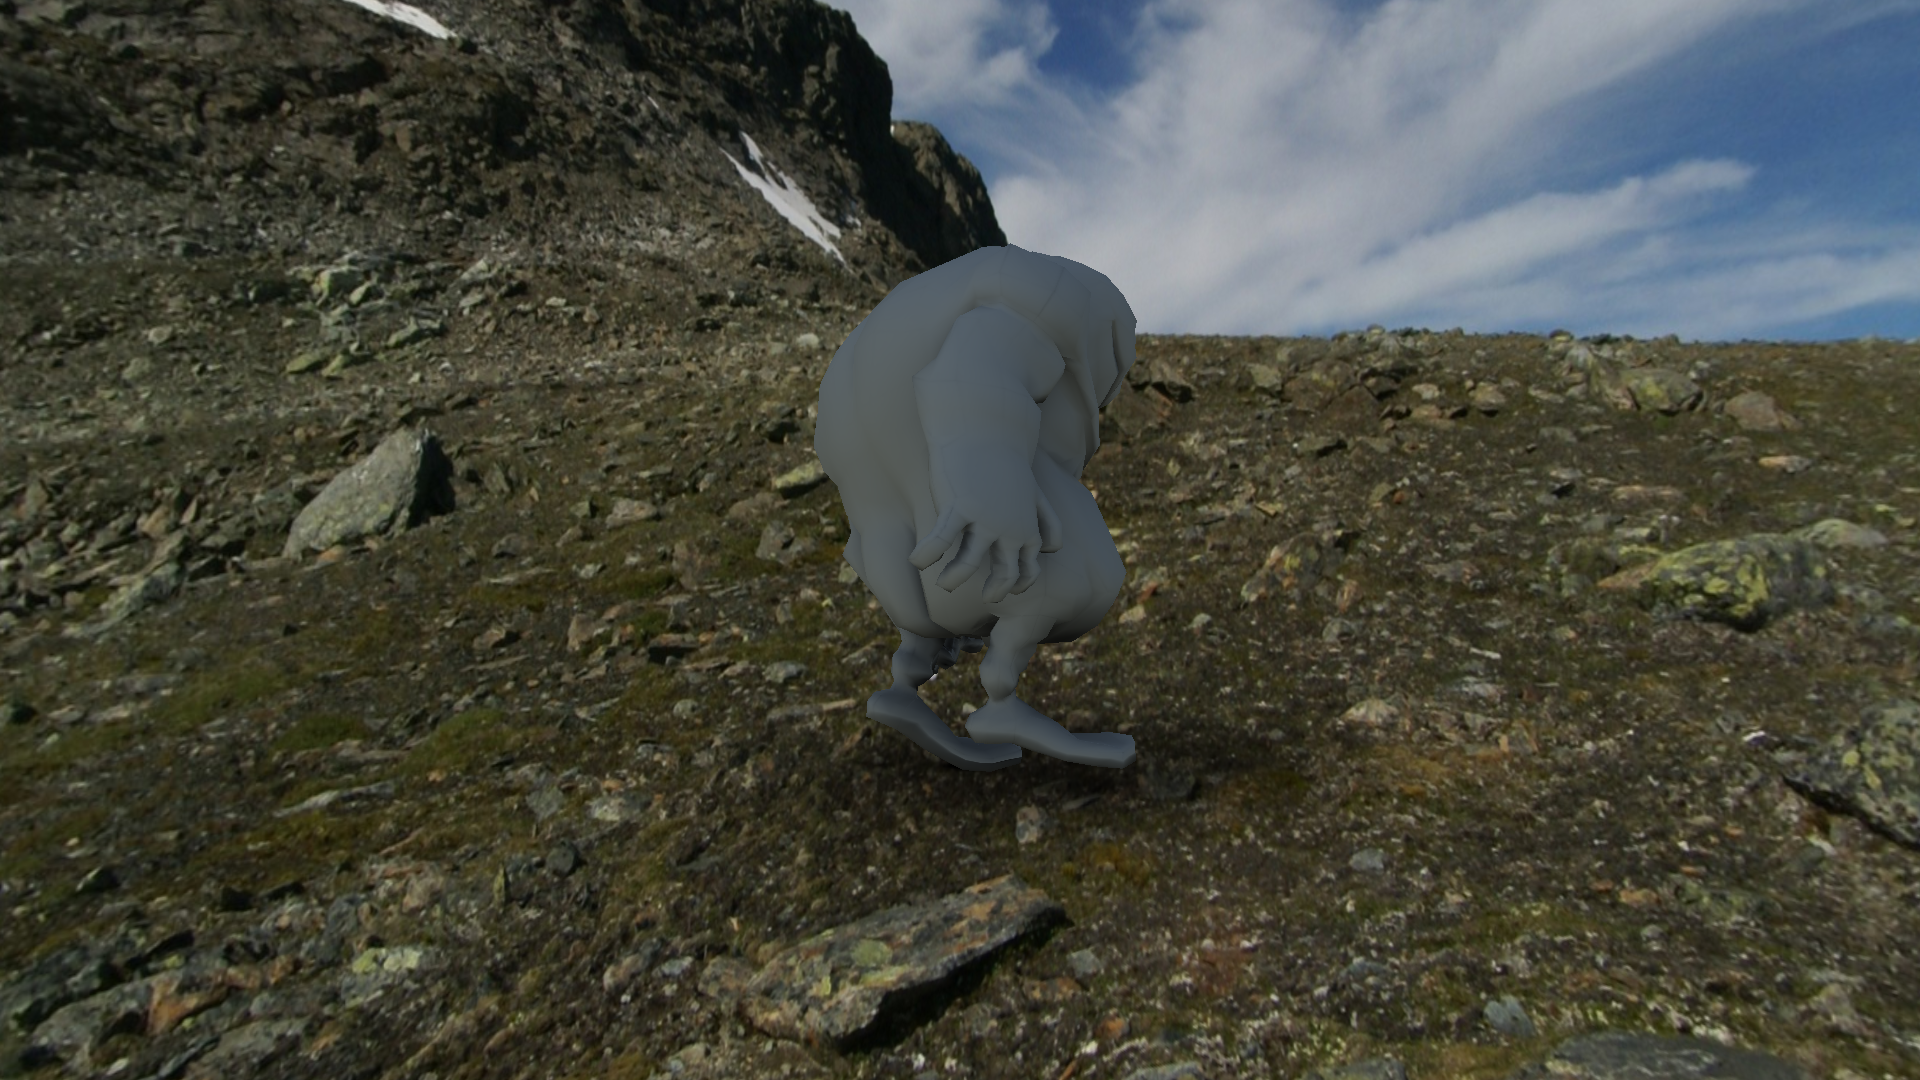
\includegraphics[width=0.45\textwidth]{\rootPath Imgs/screen/white-3.png}
		\caption{Rendu du modèle “bigguy” pour différents niveau de spécularité}
	\end{figure}
\end{frame}
\begin{frame}{Résultats du rendu}
	\begin{figure}
		\centering
			\includegraphics[width=0.45\textwidth]{\rootPath Imgs/screen/glossy-1.png}
			~
			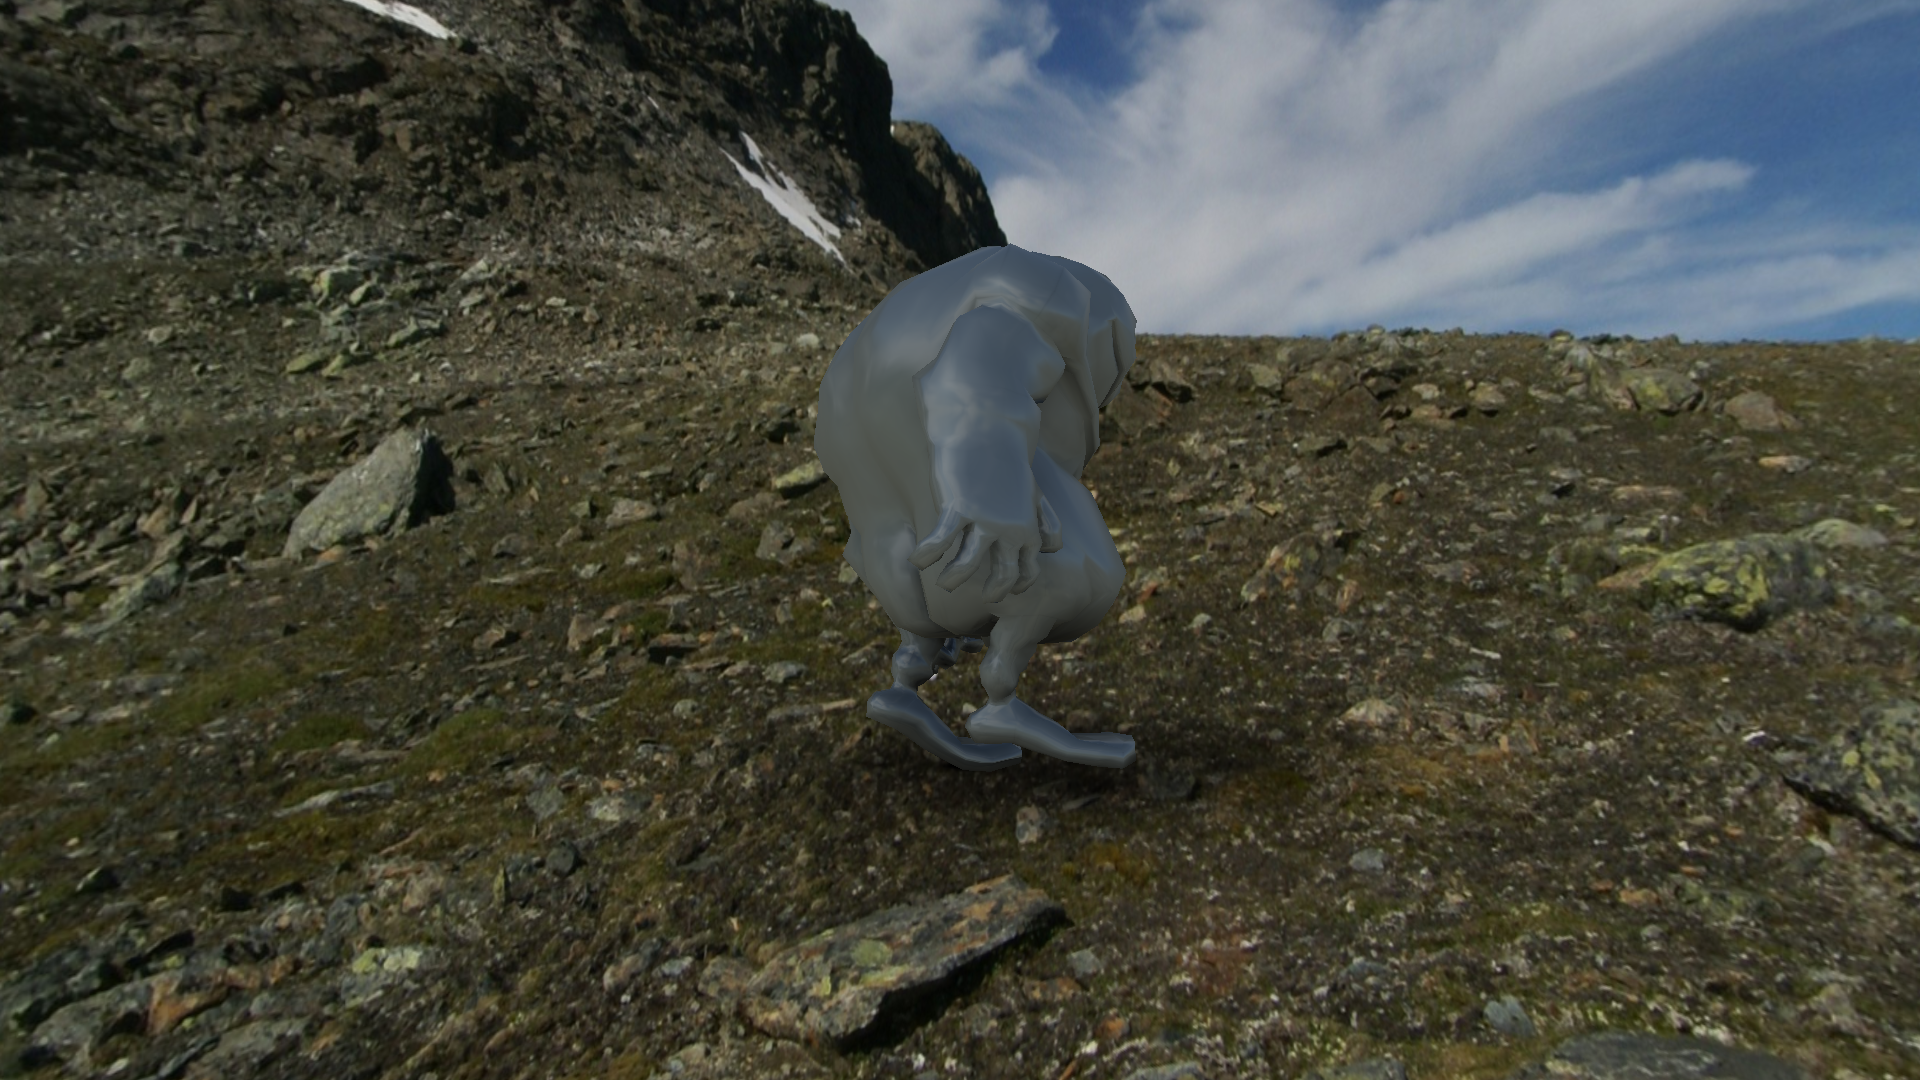
\includegraphics[width=0.45\textwidth]{\rootPath Imgs/screen/glossy-3.png}
		\caption{Rendu du modèle “bigguy” pour différents niveau de spécularité}
	\end{figure}
\end{frame}
\begin{frame}{Résultats du rendu}
	\begin{figure}
		\centering
			\includegraphics[width=0.45\textwidth]{\rootPath Imgs/screen/miror-1.png}
			~
			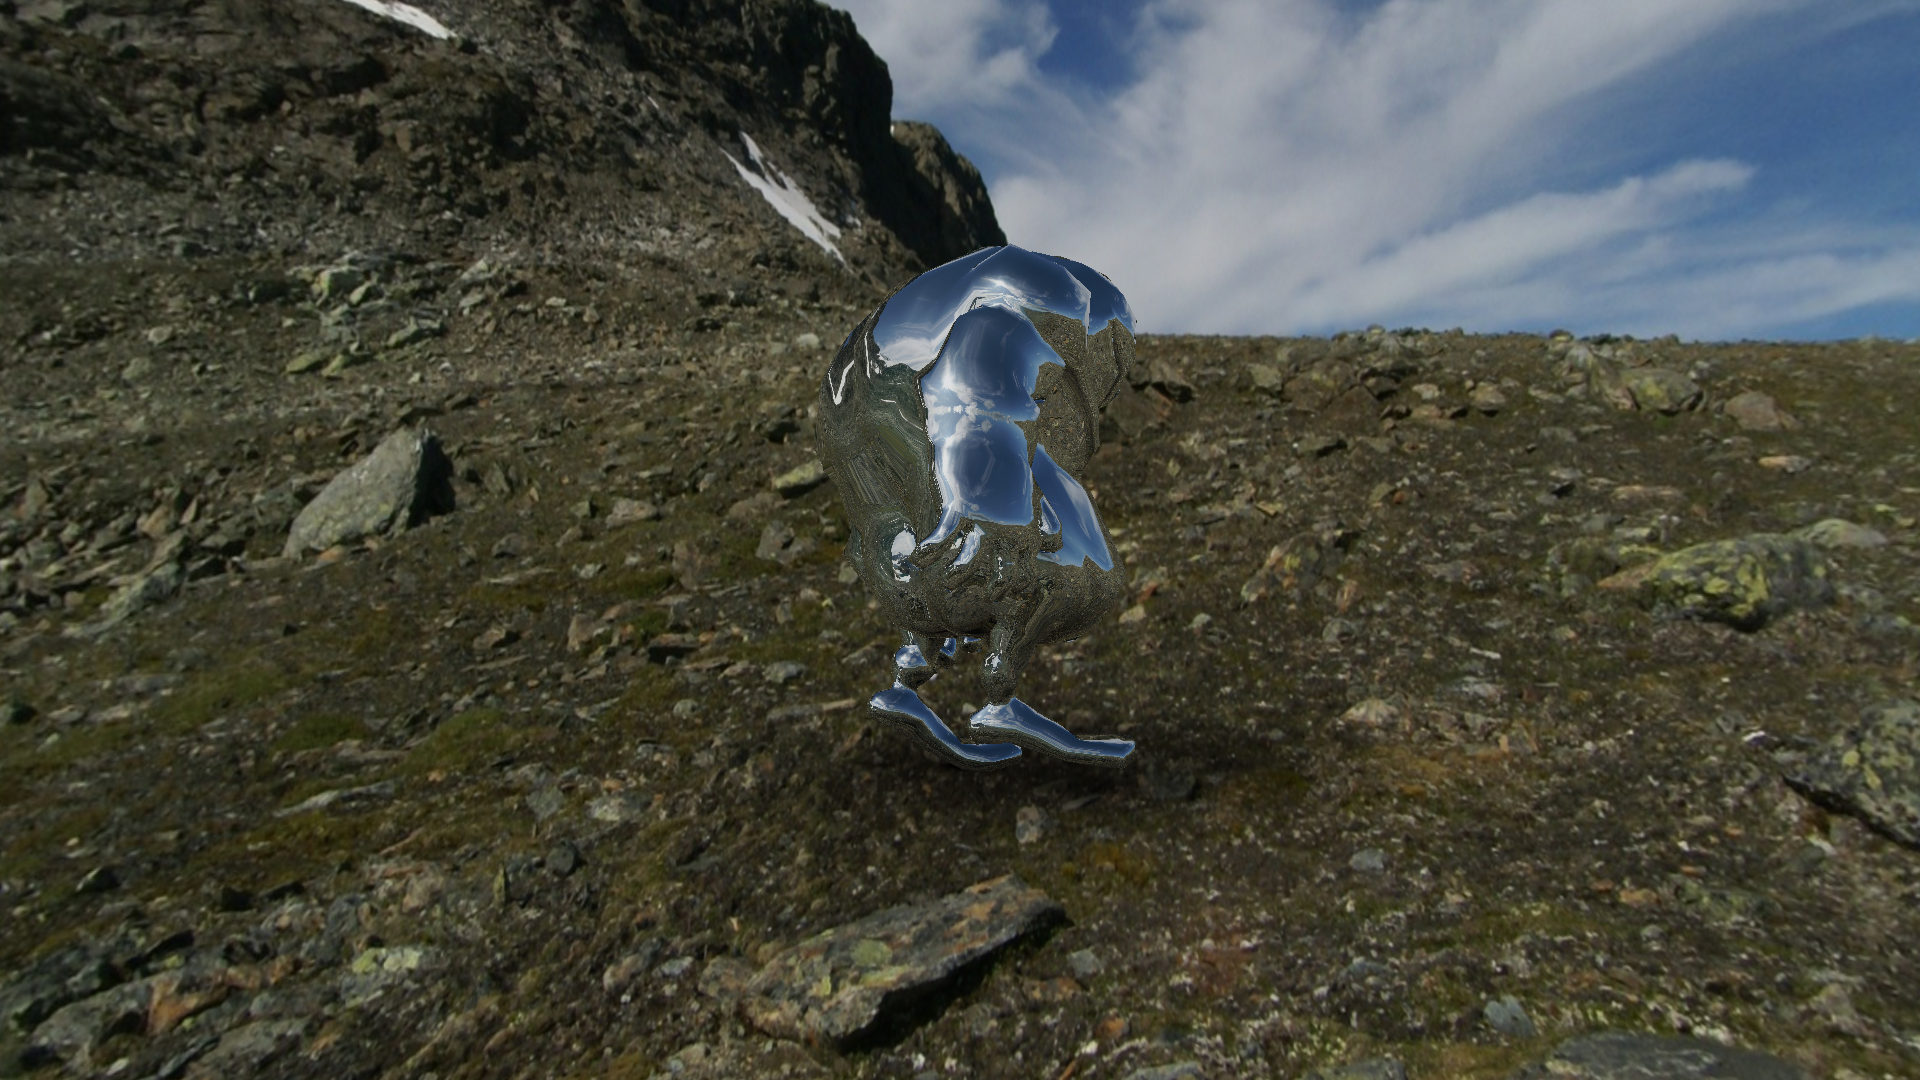
\includegraphics[width=0.45\textwidth]{\rootPath Imgs/screen/miror-3.png}			
		\caption{Rendu du modèle “bigguy” pour différents niveau de spécularité}
	\end{figure}
\end{frame}

\begin{frame}{Perspectives d'évolution}
	\begin{itemize}
		\item Envmap HDR;
		\item BRDF à micro-facettes;
		\item Modèles animés.
	\end{itemize}
\end{frame}


\begin{frame}
	\begin{itemize}
		\item Merci de votre attention
		\item Avez-vous des questions ?
	\end{itemize}
\end{frame}


\end{document}
